\chapter{超连续谱生成}
\label{ch:supercontinuum}

前面的章节解释了单个线性和非线性效应及其相互作用,并总结了它们的影响,如表~\ref{tab:NL_summary}所示。对于具有载频使得$\betag_2\lesssim 0$且$\gamma>0$的高功率脉冲,以及持续时间低于约100~fs的情况,这些效应可能同时存在。在这种情况下,脉冲的演化可能非常复杂,并将其谱宽度扩展到其初始带宽的十到二十倍~\cite{supercontinuum_original_paper}。本章通过一个超连续谱生成的例子,阐述了如何通过之前讨论的效应理解这一过程。

\begin{table}[]
\begin{adjustwidth}{-2cm}{}
\begin{tabular}{ccccc}
\hline
\textbf{效应}       & \textbf{时域表现}                                                                                      & \textbf{光谱表现}                                                                                           & \textbf{对以下情况显著}                                                                           & \textbf{相关性}                                                                                                       \\ \hline
$\alpha>0$            & 增加功率.                                                                                           & 增加功率.                                                                                             & 放大器                                                                                         & \begin{tabular}[c]{@{}c@{}}非线性效应高度\\ 依赖于功率.\end{tabular}                                            \\ \hline
$\beta_2<0$           & \begin{tabular}[c]{@{}c@{}}脉冲前端(蓝)和后端(红)\\ 各自展宽.\end{tabular}            & \begin{tabular}[c]{@{}c@{}}光谱相位\\ 随与载频的\\ 距离变化.\end{tabular} & \begin{tabular}[c]{@{}c@{}}短的NIR脉冲\\ 在二氧化硅中.\end{tabular}                             & \begin{tabular}[c]{@{}c@{}}非线性效应在\\ $\beta_2+\gamma P\approx 0$时显著.\end{tabular}                      \\ \hline
$\beta_3$             & \begin{tabular}[c]{@{}c@{}}根据符号推迟或提前\\ 非载频成分.\end{tabular}    & \begin{tabular}[c]{@{}c@{}}光谱相位与\\ 载频的\\ 距离三次方变化.\end{tabular}        & \begin{tabular}[c]{@{}c@{}}载频接近\\ 零色散频率(ZDF).\end{tabular}                            & \begin{tabular}[c]{@{}c@{}}不同频率在时域中\\ 重叠导致FWM.\\ 孤子分裂.\end{tabular} \\ \hline
自相位调制(SPM) & \begin{tabular}[c]{@{}c@{}}脉冲前缘(红)和后缘(蓝)\\ 各自偏移.\end{tabular}                     & \begin{tabular}[c]{@{}c@{}}对称\\ 展宽.\end{tabular}                                            & 高功率脉冲                                                                                  & \begin{tabular}[c]{@{}c@{}}最基本的非线性效应. \\ 首先“启动”随着\\ 功率增大.\end{tabular}            \\ \hline
自陡化       & \begin{tabular}[c]{@{}c@{}}脉冲峰值延迟\\ 到后期时间,\\ 导致陡峭的后坡.\end{tabular} & \begin{tabular}[c]{@{}c@{}}偏向高频的\\ 展宽.\end{tabular}                 & \begin{tabular}[c]{@{}c@{}}短时脉冲与载频\\ 比较.\end{tabular} & \begin{tabular}[c]{@{}c@{}}SPM的细微修正。\\ 孤子分裂.\end{tabular}                            \\ \hline
拉曼效应     & 脉冲峰值红移。                                                                                  & \begin{tabular}[c]{@{}c@{}}偏向低频的\\ 展宽.\end{tabular}                  & \begin{tabular}[c]{@{}c@{}}极短脉冲在\\ 10-100fs量级.\end{tabular}     & \begin{tabular}[c]{@{}c@{}}拉曼红移效应\\ 可以超过SPM\\ 展宽.  \\ 孤子分裂.\end{tabular}            \\ \hline
\end{tabular}
\caption{不同线性和非线性效应的影响总结。}
\label{tab:NL_summary}
\end{adjustwidth}
\end{table}

\section{案例研究}
为了模拟超连续谱的生成,使用了表~\ref{tab:SC_params}中的参数。生成的超连续谱如图~\ref{fig:SC_combined}所示。图~\ref{fig:SC_combined} c)中的光谱表明,脉冲在前1~m的传播过程中经历了SPM效应,而图~\ref{fig:SC_combined} b)表明,孤子分裂发生在随后的区域。高功率脉冲具有比初始脉冲小得多的持续时间,它沿着抛物线向后延伸,形成一个拉曼孤子,并不断发生红移。线性"走离"的低功率光可能是由FWM生成的,这一过程发生在分裂的孤子与初始脉冲残余部分重叠时。有关此超连续谱的详细分析,请参阅\href{https://youtu.be/-GDsMDpC3oA}{此视频教程}。

\begin{table}[]
\centering
\begin{tabular}{cc}
\textbf{参数}                      & \textbf{数值}                                  \\ \hline
时间点数                           & $2^{14}$                                          \\ 
时间分辨率 {[}fs{]}                & 1.8                                             \\ \hline
脉冲类型                              & Sech                                            \\ 
持续时间 {[}fs{]}                       & 166.79                                          \\ 
峰值功率 {[}W{]}                      & 50                                              \\ 
载频 {[}THz{]}                 & 282.823 (=1060~nm)                         \\ \hline
$\alpha$ {[}dB/km{]}                    & 0                                               \\ 
$\betag_2$ {[}s\textasciicircum{}2/m{]} & -3.051721e-27                                   \\ 
$\betag_3$ {[}s\textasciicircum{}3/m{]} & 7.29029e-41                                     \\ 
$\betag_4$ {[}s\textasciicircum{}4/m{]} & -1.08817e-55                                    \\ 
$\betag_5$ {[}s\textasciicircum{}5/m{]} & 2.8941e-70                                      \\ 
$\betag_6$ {[}s\textasciicircum{}6/m{]} & 4.8348e-89                                      \\ 
$\betag_7$ {[}s\textasciicircum{}7/m{]} & -1.1464e-113                                    \\ 
$\betag_8$ {[}s\textasciicircum{}8/m{]} & 1.8802e-128                                     \\ 
$\betag_9$ {[}s\textasciicircum{}9/m{]} & -1.5054e-143                                    \\ 
$\gamma$ {[}1/W/m{]}                    & 0.09                                            \\ 
自陡化                         & 开启                                              \\ 
拉曼模型                             & 方程~\ref{eq:raman_basic}
\end{tabular}
\caption{用于生成超连续谱的模拟参数,取自~\cite{supercontinuum_paper}}
\label{tab:SC_params}
\end{table}

\begin{figure}
    \centering
    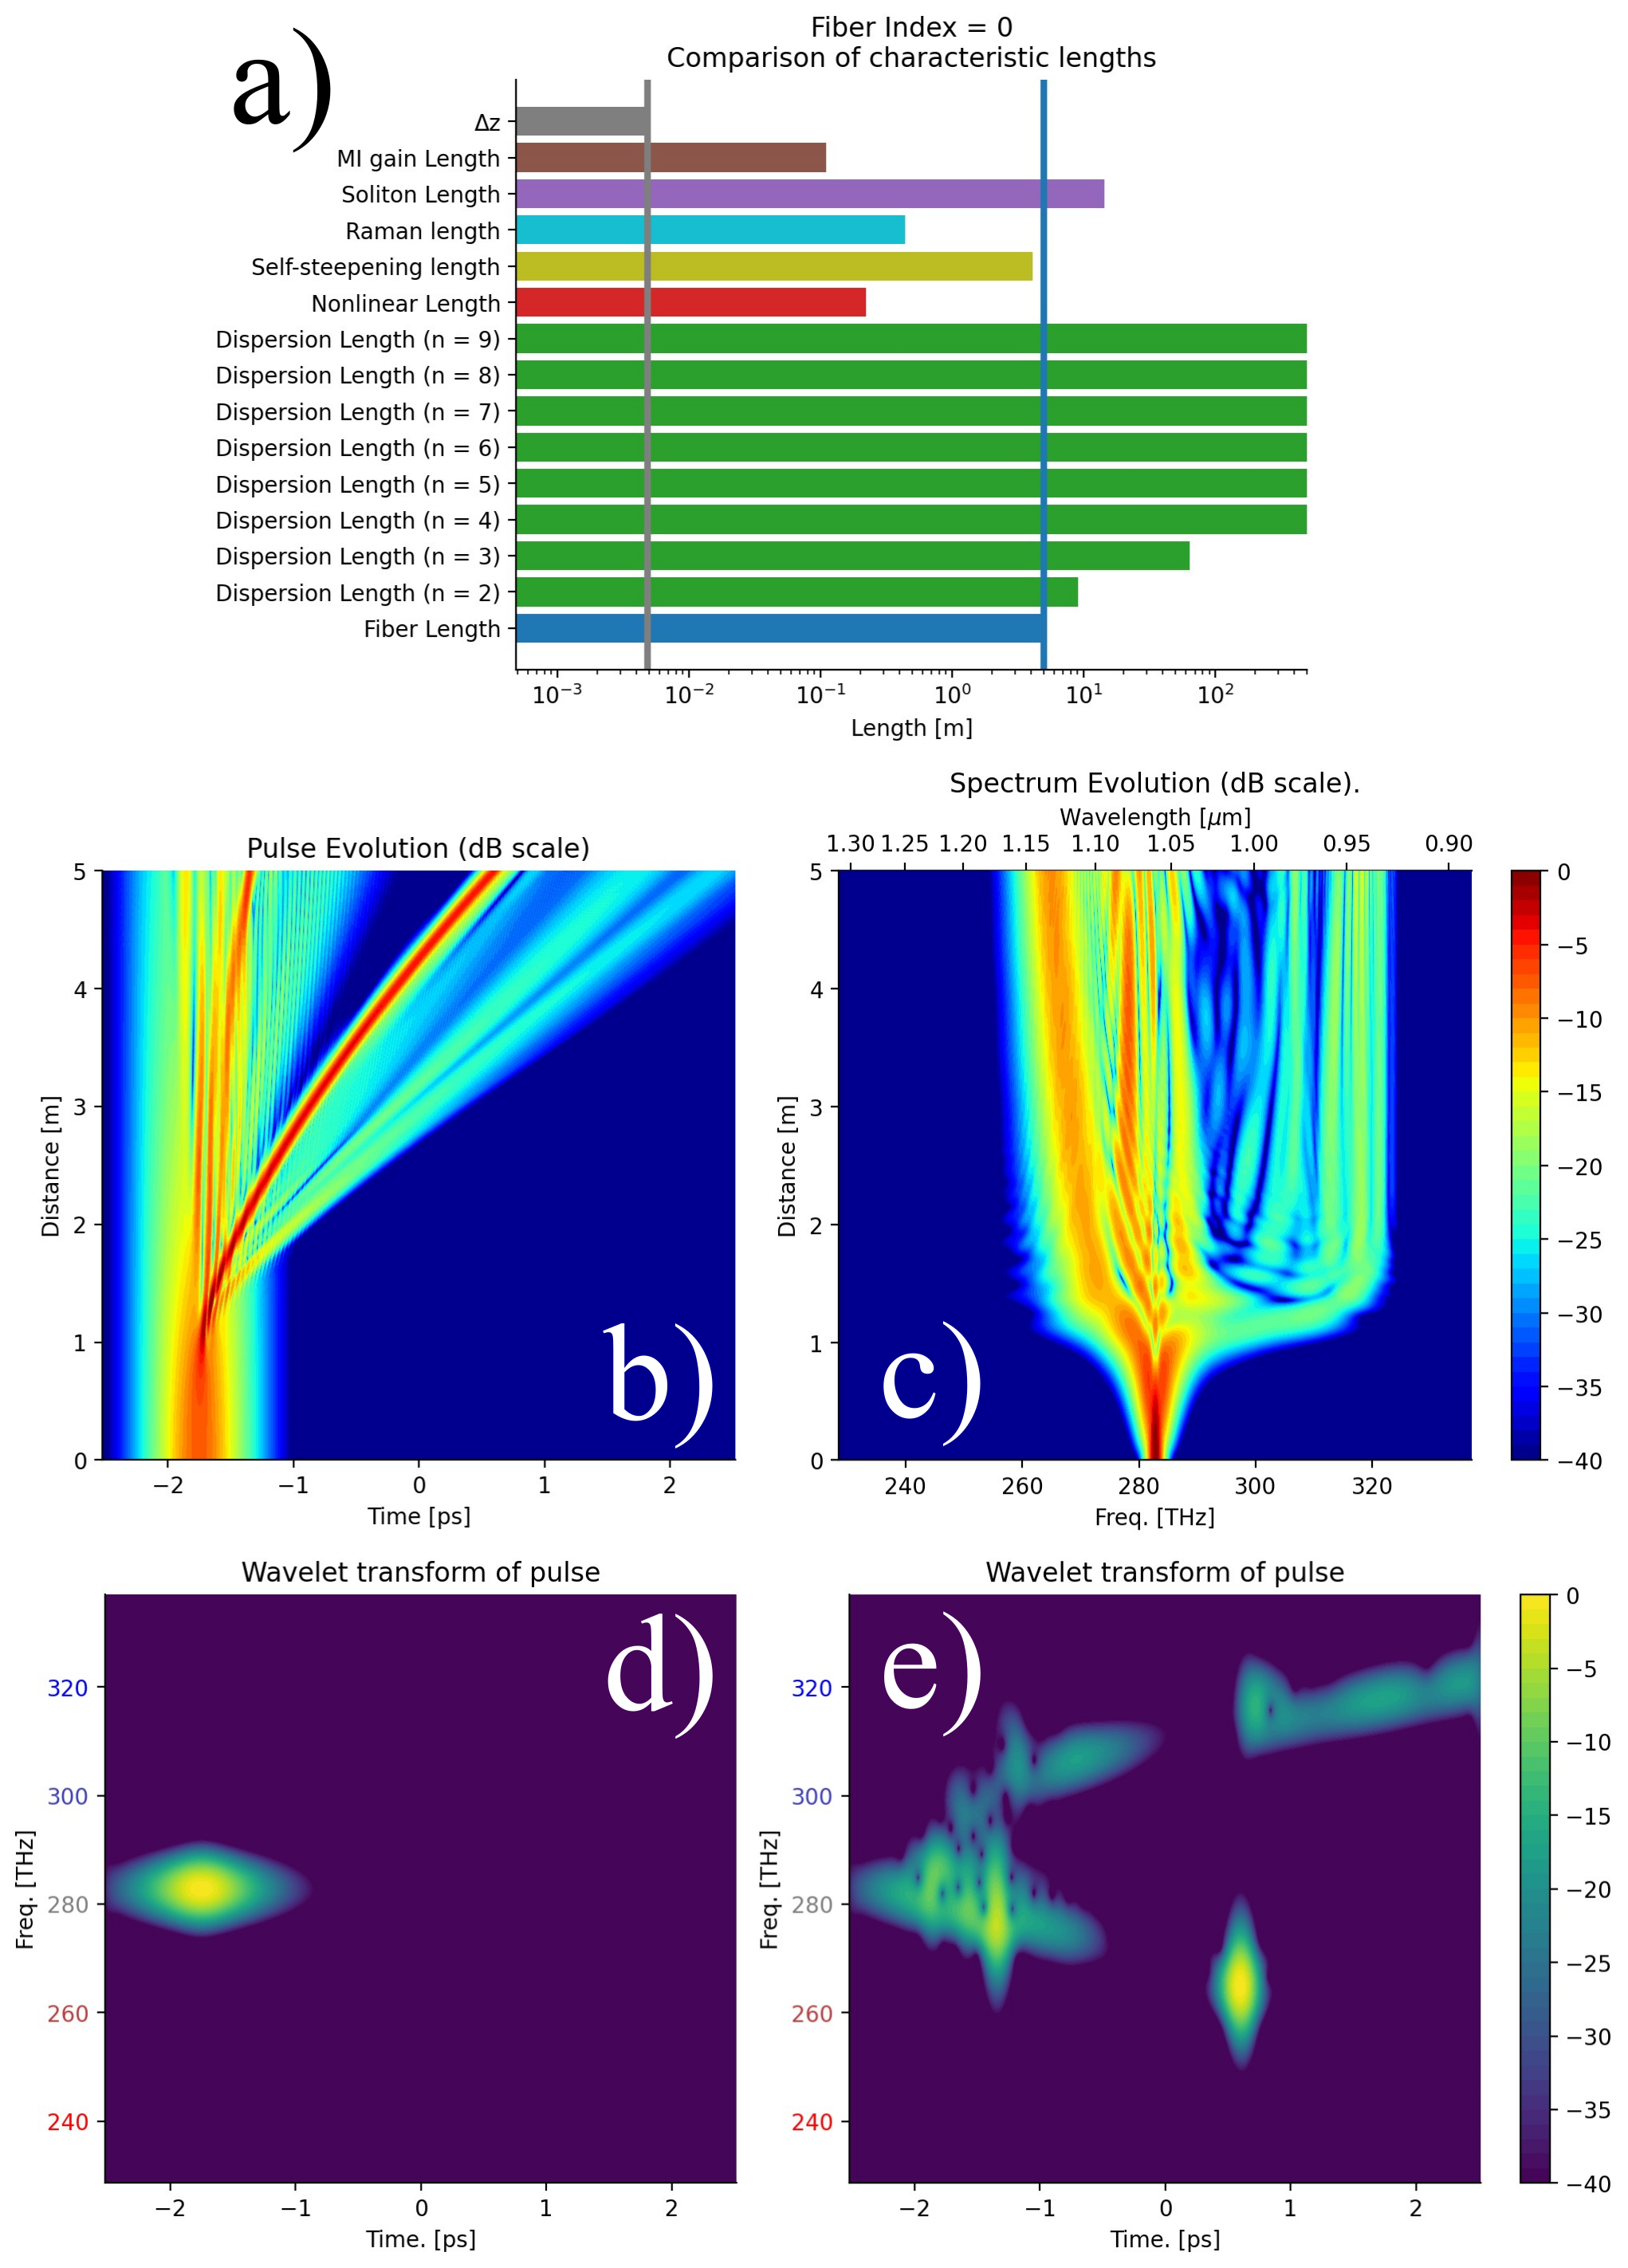
\includegraphics[width=0.9\linewidth]{figures/SC_combined.png}
    \caption{a) 使用表~\ref{tab:SC_params}中列出的参数比较特征长度。具有短特征长度的效应将首先变得显著。b) 脉冲的时间演化,显示在约1~m的距离处发生孤子分裂,之后是FWM并生成拉曼孤子,逐渐向后延伸。c) 脉冲的光谱演化。d) 初始时刻$z=0$的光谱图。e) $z=5$~m时的光谱图。}
    \label{fig:SC_combined}
\end{figure}

\section{你的实验}
为了进一步探索图~\ref{fig:SC_combined}中模拟的超连续谱特性,请打开生成该图的\href{https://colab.research.google.com/drive/1HvA8F8yzEq-9fahuI4z2KhT-YhdRAXgt?usp=sharing}{Colab笔记本},并进行以下实验,解释脉冲及其光谱演化的不同。每次实验前,请写下你对模拟结果的预期,以便与实际结果进行对比。请注意,在每次实验前“重置”参数到默认值:

\begin{enumerate}
\item \textbf{无非线性效应}。当前模拟使用了$\gamma>0$。将其改为$\gamma=0$。结果是否表明非线性效应对脉冲的时间演化有重要影响?

\item \textbf{无自相位调制效应}。当前模拟考虑了自相位调制的影响。关闭此效应后,观察其对结果的影响。

\item \textbf{负$\alpha$值}。当前模拟中使用$\alpha=0$。将其改为$\alpha=-1$~dB/m。观察该修改对结果的影响。

\item \textbf{正的$\betag_2$值}。当前模拟中使用$\betag_2<0$。将$\betag_2$的符号改为正值。

\item \textbf{仅$\betag_2<0$}。当前模拟中使用了$\betag_n\neq 0$($n>2$)。将$\betag_n = 0$($n>2$),运行模拟并解释脉冲及其光谱演化的变化。

\item \textbf{负$\betag_3$值}。当前模拟中使用$\betag_3>0$。将$\betag_3$改为正值。注意:为了确保正确绘制时间演化图,可能需要将时间偏移从-1.75~ps改为+1.75~ps。你能解释为什么当$\betag_3<0$时不会出现拉曼孤子吗?提示:使用公式~\ref{eq:ZDF}计算零色散频率并考虑符号变化对其的影响。

\item \textbf{修改拉曼模型}。当前模拟使用了方程~\ref{eq:raman_basic}来建模拉曼效应。根据笔记本中的提示,使用方程~\ref{eq:raman_new}、方程~\ref{eq:Raman_exact}或$f_R=0$来修改模型。
\end{enumerate}
